\usepackage[utf8]{inputenc}
\usepackage{listings}
\usepackage{textcomp}
\usepackage{fancyvrb}

\title{Exploration Oriented Programmming Nitpicks}
\subtitle{REPL to Production}
\author{Moshe Zadka -- https://cobordism.com}
\date{North Bay Python 2018}
 
\begin{document}
 
\begin{titlepage}
\maketitle
\end{titlepage}

\frame{\titlepage}

Jupyter has brought back a new style of development:
what I like to call
"exploration-oriented programming".
Inside an interactive environment,
we intermix writing code
and running it,
in a persistent process --
with persistent memory,
persistent files and
everything else.
We modify our code as needed,
running it to
see what happens.

When I was a kid,
literally a six year old boy,
I simply called this
"programming".
I had no idea that for "proper"
programming,
you have to edit text files in an integrated development environment,
hit the "compile and debug" button,
set break points,
then trash the process,
modify the code and start again.

\begin{frame}[fragile]
\frametitle{LOGO}

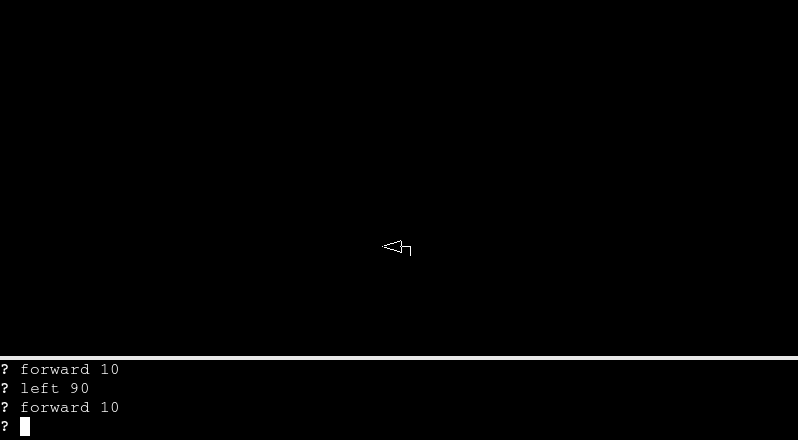
\includegraphics[height=7cm,width=10cm]{logo.png}

\end{frame}


I had my LOGO environment,
where I would write a function,
then run it and see what it did to the screen.
Then I would edit it,
exit the internal editor,
and the screen still had whatever I draw on it earlier.
I would run the function again.

\begin{frame}
\frametitle{GW-Basic}

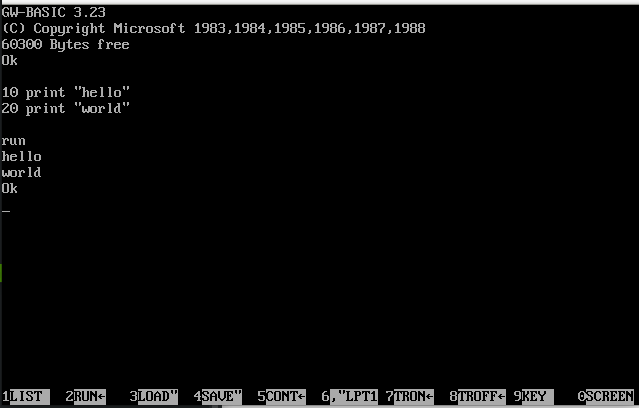
\includegraphics[height=7cm,width=10cm]{gwbasic.png}

\end{frame}

Then I grew up,
and I was a big kid,
seven years old.
I had my GW-Basic environment.
The program was a list of lines.
I could run it,
and it would run in a global namespace.
I could specify
"run starting at line 150",
so I could run only specific parts.
I could also execute lines of code directly.

If this was in graphical mode,
the graphics would be persisted between runs.

When I was eleven,
I was introduced to the magical world of Turbo C++.
You would write reams of code.
Then you would run "compile and run",
which inevitably crash.
Then you would run "compile and debug",
set a breakpoint,
then step carefully until you found out which variable was wrong.
Then you would exit all that careful local state,
hopeful that you knew what was wrong.
You edited the code.
You ran "compile and debug".
It would,
inevitably, crash.

I fell out of love with programming until,
in my 20s,
I met the Python repl.

\begin{frame}
\frametitle{Python REPL}

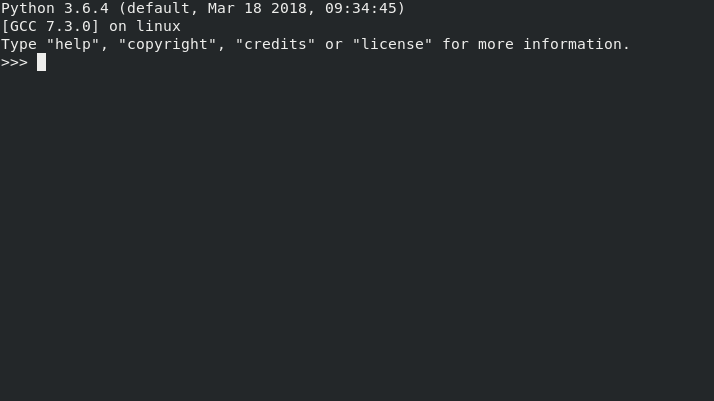
\includegraphics[height=7cm,width=10cm]{python-repl.png}

\end{frame}

It was not as cool as LOGO,
or as GW-Basic:
but at least it had the basics,
the ability to iterate through code.
Imagine my frustration when,
after getting a for loop wrong,
I had to up-arrow roughly one million times to
fix it.

Enter IPython:


\begin{frame}
\frametitle{IPython REPL}

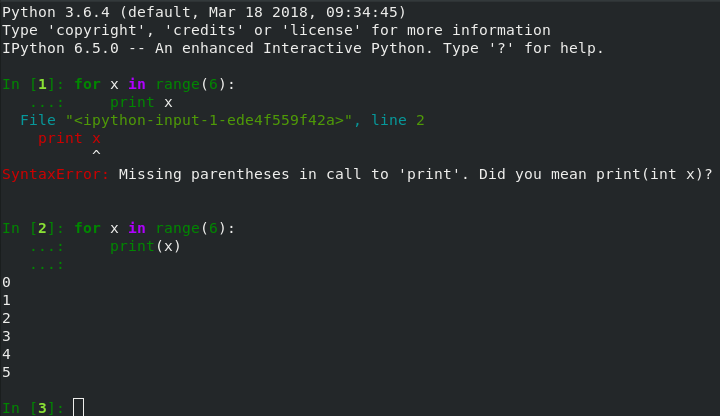
\includegraphics[height=7cm,width=10cm]{ipython.png}

\end{frame}

Sadly,
inline persistent graphics
were a thing of the past.

\begin{frame}
\frametitle{Jupyter}

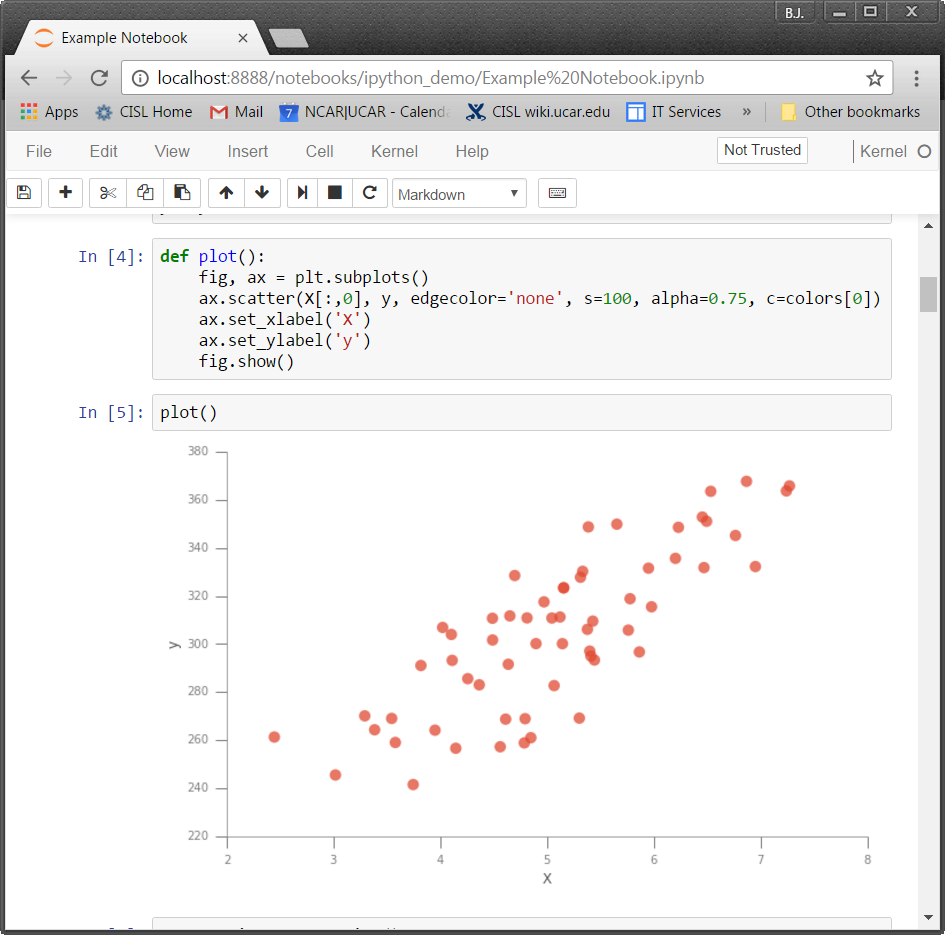
\includegraphics[height=7cm,width=10cm]{jupyter-notebook-page.png}

\end{frame}

After many years,
IPython Notebooks,
later relaunched as "Jupyter",
brought back a graphical,
interactive,
persistent environment.

\begin{frame}
\frametitle{What is Jupyter?}

\begin{itemize}
\item Web interface
\item Kernel
\item Persistent history
\item Other goodies!
\end{itemize}

\end{frame}

Jupyter is a collection of parts that works to create that environment.
That includes the web server,
the kernel that runs Python,
a file format to save the history in
(spoiler: those are the notebooks)
and other goodies:
in fact,
Jupyter has a built-in terminal and editor,
so it's a complete IDE in one.

\begin{frame}
\frametitle{Kernel}

\begin{itemize}
\item Handles snippets
\item In-memory state
\item Semi-disposable
\item Tornado event loop
\end{itemize}

\end{frame}

The kernel is the "heart":
it is a Python server
that receives snippets,
executes them in its internal namespace,
and then sends back the results.

It uses the tornado event loop internally,
and since Python is pretty loose about things,
this fact is exposed to the end user.

Jupyter makes it easy to recycle the kernel,
in case we do not *want* the persistent
in-state memory
and want to start from scratch.

\begin{frame}[fragile]
\frametitle{Magic}

\begin{lstlisting}
%%pdb
\end{lstlisting}

\begin{lstlisting}
%% capture output
...
\end{lstlisting}

\end{frame}

The IPython "kernel" also knows some "magic" sequences.
This can do anything from launching into a debugger
to how to capture the output.

By the way,
if you use IPython as a REPL,
the same magic commands work.
If you are not using IPython as your REPL,
you should start!

\begin{frame}[fragile]
\frametitle{Managing Kernels}

\begin{lstlisting}
def add_to(kernel_venv, jupyter_venv):
    python = os.path.join(kernel_venv, 'bin', 'python')
    name = os.path.basename(kernel_venv)
    subprocess.check_call([python, '-m',
                           'pip', 'install', 'ipykernel'])
    subprocess.check_call([python, '-m',
                           'ipykernel', 'install',
                           '--name', name,
                           '--display-name', name,
                           '--prefix', venv])
    jupyter = os.path.join(jupyter_venv, 'bin', 'jupyter')
    spec = os.path.join(venv, 'share/jupyter/kernels', name)
    subprocess.check_call([jupyter, 'kernelspec', 'install', spec])
\end{lstlisting}
\end{frame}

One server can support multiple virtual environments.
Assuming you're doing the reasonable thing and installing
Jupyter server itself in a virtual environment,
the instructions for how to add a virtual environment
to an existing servers are not clear.

However,
once followed,
this becomes a powerful tool:
create a new virtual environment,
and it is already available in the pre-existing browser session.
Assuming that,
like everybody these days,
you are working on some microservice architecture,
this is a useful tool to have each microservice in its own virtual environment,
but manage them together and easily switch between them.

\begin{frame}
\frametitle{Security Model}

\begin{itemize}
\item Opaque security token
\item By default, listen only on localhost
\end{itemize}

\end{frame}

When first running Jupyter,
it will generate a random token and try to launch your browser.
Assuming everything is simple, this will work.
It will also print out a URL.
Assuming everything is kinda simple, this will work.
If all else fail,
the URL contains a token.
If you connect to the server,
it will ask for a token,
and then authenticate you.

This works well when your networking set-up is exotic:
maybe you have a proxy to your AWS VPN which sits behind an oauth proxy,
or,
even worse,
you're running Jupyter in a container on your laptop.

\begin{frame}
\frametitle{Notebooks}

\begin{itemize}
\item Editable history
\item Inputs and outputs
\item Code, not state
\end{itemize}

\end{frame}

Notebooks contain the history of your project...
almost.
Unlike real history,
you can go back and edit any cell.
This is useful for cleaning up for presentation,
though it can be a problem when reading a notebook straight through.
The use of a notebook is not as a *proof* a procedure
was followed and results were given:
it's a recipe for getting the result,
and an editable one at that.

The notebook has the inputs and the outputs in it,
but none of the memory state.
It maps,
pretty much,
to what is on the screen.


\begin{frame}[fragile]
\frametitle{Notebooks from the Inside}

\begin{lstlisting}
{
 "cells": [
  { "cell_type": "code",
   ...
    "source": ["1 + 1"]
  }
 ]
 "nbformat": 4,
 "nbformat_minor": 1
}
\end{lstlisting}

\end{frame}

A notebook,
from the inside,
is just a JSON file.
It has some metadata,
and an array of "cells",
which include the type of cells,
as well as the source
and possibly the output.

7 minute mark

\begin{frame}[fragile]
\frametitle{Global namespace}

\begin{lstlisting}[frame=single]
some_thing = 15
\end{lstlisting}

\begin{lstlisting}[frame=single]
some_thing * 2
\end{lstlisting}

\begin{lstlisting}[frame=single]
30
\end{lstlisting}

\end{frame}

Remember that the namespace for the notebook is global:
be cautious and thoughtful when setting global variables.
This is no different than most Python modules,
but there is more temptation to randomly litter the global
namespace with ad-hoc values for easy testing.
There is less need than you think:
you can run a function on a literal directly for tests.
When defining global variables for ad-hoc reasons,
name them in a way that is unlikely to be shadowed
by local variables in functions,
or your code will be surprisingly fragile.

\begin{frame}[fragile]
\frametitle{Redefining functions}

\begin{lstlisting}[frame=single]
def foo(a):
    return 2 * a
\end{lstlisting}

\begin{lstlisting}[frame=single]
foo(10)
\end{lstlisting}

\begin{lstlisting}[frame=single]
20
\end{lstlisting}

\begin{lstlisting}[frame=single]
def foo(a):
    return 3 * a
\end{lstlisting}

\begin{lstlisting}[frame=single]
30
\end{lstlisting}

\end{frame}

Redefining functions is sometimes useful.
It's a good habit to edit them in a new cell,
although for small modifications,
sometimes editing the cell is fine.
This is no different from updating globals,
although in these cases,
you will want to remove all definitions
but one from your notebook before the end.

\begin{frame}[fragile]
\frametitle{Immutable data structures}

\begin{lstlisting}[frame=single]
from pyrsistent import v
a = v(1, 2, 3)
\end{lstlisting}

\begin{lstlisting}[frame=single]
def increase_head(stuff):
    return stuff.set(0, stuff[0] + 1)
increase_head(a)
\end{lstlisting}

\begin{lstlisting}[frame=single]
pvector([2, 2, 3])
\end{lstlisting}

\begin{lstlisting}[frame=single]
def increase_tail(stuff):
    return stuff.set(-1, stuff[-1] + 1)
increase_tail(a)
\end{lstlisting}

\begin{lstlisting}[frame=single]
pvector([1, 2, 4])
\end{lstlisting}

\end{frame}

Using immutable data structures means you can run
reasonably efficient functions which transform the data,
but,
if they have a problem,
you can edit them and try again.
The pyrsistent library defines efficient immutable data structures.
This is also a good way to code,
so we can just keep our coding style as is.

\begin{frame}[fragile]
\frametitle{Verification as testing}

\begin{lstlisting}[frame=single]
# test
x = [1, 2, 3]
y = increase_tail(x)
assert_that(y[2], is_(5))
\end{lstlisting}

\begin{lstlisting}[frame=single]
...
AssertionError: 
Expected: <5>
     but: was <4>
\end{lstlisting}

\end{frame}

Using a library such as PyHamcrest
(my favorite assertion library)
we can verify that a function does the right thing.
It will raise a nice,
readable,
exception if the function fails:
in that case, we can edit the function cell,
execute it,
and re-execute the test.

Explicitly marking such verification steps as "tests"
means that if we want to use this Notebook as code,
we know to skip over them if we are using it as a library,
or to run them all if we want to test the Notebook --
for example, in CI.

\begin{frame}[fragile]
\frametitle{Classes}

\begin{lstlisting}[frame=single]
@attr.s(frozen=True)
class Point:
     x = attr.ib()
     y = attr.ib()
\end{lstlisting}

\end{frame}

The way to incrementally build classes it to make the classes
data-first.
Think about their data before you think about their behavior.
Of course, we're not going to forget about immutability.
Immutability good!

\begin{frame}[fragile]
\frametitle{Dispatching}

\begin{lstlisting}[frame=single]
@singledispatch
def abs(thing):
    raise NotImplementedError("Cannot absolute value", thing)
\end{lstlisting}

\begin{lstlisting}[frame=single]
@abs.register(Point)
def abs(pt):
    return (pt.x**2 + pt.y**2) ** 0.5
\end{lstlisting}

\end{frame}

We can incrementally add "methods" to classes with singledispatch.
It is an awesome library for retroactively adding methods to classes.
I often recommend using it anyway,
since it properly namespaces methods.
This is one additional reason to use it.

\begin{frame}[fragile]
\frametitle{Version control}

\begin{lstlisting}
   "execution_count": 1,
   "outputs": [
    {
     "data": {
      "text/plain": [
       "2"
      ]
     },
     "execution_count": 1,
     "metadata": {},
     "output_type": "execute_result"
    }
   ],
\end{lstlisting}

\end{frame}

If notebooks become a source material,
checking them in is useful.
However,
that often causes spurious diffs.
The outouts,
and the execution counts,
are intermingled with the source code.
While this does not stop one common use case,
checking the notebooks as a backup strategy,
it does means that reviewing the diffs
in a pull requests or,
even worse,
having a three way merge,
become much more complicated than needs be.

\begin{frame}[fragile]
\frametitle{Cleaning outputs}

\begin{lstlisting}
with open("something.ipynb") as fpin:
    data = fpin.read()
    parsed = json.loads(data)
    for cell in parsed["cells"]:
        del cell["output"]
        del cell["execution_count"]
with open("something_cleaned.ipynb") as fpout:
    fpout.write(json.dumps(parsed))
\end{lstlisting}

\end{frame}

One easy solution is to write an "output scrubber".
This is an example,
that has limited,
but non-zero uses.

\begin{frame}
\frametitle{Cleaning outputs}

\begin{itemize}
\item Pre-commit hook
\item Test in CI that re-cleaning gives same result
\item Code review the cleaned file
\end{itemize}

\end{frame}

For example,
even though it's not a valid notebook,
it does give us a path to review the notebook.
We clean before we commit,
and commit the result.
This,
of course,
depends on client behavior,
so we cannot depend on that.
Instead,
we have CI checking that cleaning the checked-in notebook
yields the same result as the checked-in clean notebook,
and fail otherwise.
Doing it in CI means we prevent merges that have not been scrubbed
properly.
The next step is to follow the rule that we only {\em review}
the cleaned notebook's diff.
Even though we'll {\em use} the non-clean notebook,
this process ensures we are not missing any important
differences.

\begin{frame}[fragile]

\frametitle{Lint}

\begin{lstlisting}
% jupyter nbconvert --to=python something.ipynb
% flake8 something.py
\end{lstlisting}

\end{frame}

Running a linter is even easier:
in CI,
or via something like :code:`tox`
or :code:`nox`,
we can convert our notebooks to Python,
and run lint against those.
The downside,
unfortunately,
is that line numbers get jumbled.

\begin{frame}[fragile]
\frametitle{Test}

\begin{lstlisting}
with open("something.ipynb") as fpin:
    notebook = json.loads(fpin.read())
with open("something.py", "w") as fpout:
    for cell in notebook["cells"]:
        if ("# pragma: interactive-only" in
            cell["source"]):
            continue
        fpout.write(f"\n{cell['source']}\n")
subprocess.check_output(["pytest", "something.py"])
\end{lstlisting}

\end{frame}

We can improvise something to directly run our notebook,
with the exception of some "interactive-only"
tests.
If we have written "verifications" inside the notebook
that are functions named "test" and use something like
PyHamcrest,
this will be useful to run automatically.


\begin{frame}[fragile]
\frametitle{Custom diff}

\begin{lstlisting}
# Suitable for use as "git difftool"
def to_lines(fname):
    with open(fname) as fpin:
        contents = json.loads(fpin.read())
    for i, cell in enumerate(contents["cells"]):
        yield f'Cell {i}'
        yield from cell["source"].splitlines()
sys.stdout.writelines(difflib.contextdiff(
    to_lines(os.environ['LOCAL']),
    to_lines(os.environ['REMOTE']),
    'a/' + os.environ['MERGED'],
    'b/' + os.environ['MERGED'],
))
\end{lstlisting}

\end{frame}

We can take advantage of Python difflib,
and the ability of version control systems to
have custom diff tools,
in order to write a custom diff tool.
While it would not help reviewing on GitHub,
it does help local comparison work.

\begin{frame}
\frametitle{Custom merge}

\begin{itemize}
\item Clean
\item Merge
\item Add dummy output
\item (Beyond current scope)
\end{itemize}

\end{frame}

It is possible to write a custom merge tool,
as well,
that understands cells and notebooks.
This is definitely not going to fit on a slide,
even with significant simplifications.
However,
it can be worth it.

21 minute mark

\begin{frame}[fragile]
\frametitle{Importing Notebooks}

\begin{lstlisting}
@attr.s(frozen=True)
class NotebookLoader:
    contents = attr.ib()

    def create_module(self, spec):
        return importlib.util.module_from_spec(spec)

    def exec_module(self, module):
        for cell in json.loads(contents)["cells"]:
            if cell.starts_with("#pragma: module"):
               exec(cell, module.__dict__)
\end{lstlisting}

\end{frame}

Python has custom import hooks nowadays.
They are a little non-trivial to understand at first,
but reasonably straightforward to write.
In this case,
we take all cells that have the "module" pragma,
and execute them to make a module.
There are,
of course,
other approaches,
but this is enough for a bare-bones notebook imports.


\begin{frame}[fragile]
\frametitle{Finding Notebooks}

\begin{lstlisting}
class NotebookFinder(object):
 
    def find_module(self, fullname, path=None):
        if path is None:
            return None
        name = fullname.split('.')[-1] + '.ipynb'
        if not resources.is_resource(path, name):
            return None
        return NotebookLoader(resources.read_text(path, name))

import sys
sys.meta_path.append(NotebookFinder())
\end{lstlisting}

\end{frame}

The other part of the import machinery is a finder.
This finder assumes notebooks will always be a part of a package.
This simplifies the finding logic, and makes sense.

\begin{frame}[fragile]
\frametitle{Integrating with packages}

\begin{lstlisting}
somepackage/
           __init__.py
             import sys
             sys.meta_path.append(NotebookFinder())
           module.ipynb
\end{lstlisting}

\end{frame}

The file structure that results is fairly straightforward.
It's probably a good idea to check if a NotebookFinder 
is already in the meta path,
but I am going to leave these implementation details out.
The trick of making sure that the loader is correctly set up
in the dunder-init file,
however,
is the crux here:
this allows just distributing a regular package,
without any exotic installation instructions.

\begin{frame}[fragile]
\frametitle{Producing documentation}

\begin{lstlisting}
.. automodule package.module
   :members:
\end{lstlisting}

\end{frame}

Since Sphinx works by importing modules,
we can create documentation using Sphinx the same
way we do with any other package.

\begin{frame}[fragile]
\frametitle{Producing documentation}

\begin{lstlisting}
with open("something.ipynb") as fpin:
    notebook = json.loads(fpin)
with open("something.md", "w") as mdout:
    for cell in notebook["cells"]:
        if cell["cell_type"] != "markdown":
            continue
        mdout.write(cell["source"])
\end{lstlisting}

\end{frame}

We can also spit all markdown cells into a file,
and put that in.
If we do it in the right order,
and set up all the commands with something like
tox or nox,
we can have our nice documentation produced by our build process.
Luckily,
Sphinx supports markdown semi-natively!


\begin{frame}[fragile]
\frametitle{Building wheels}

\begin{lstlisting}
MANIFEST.in
  include *.ipynb
\end{lstlisting}

\end{frame}

In order to build wheels,
all we have to do is write the right thing in the MANIFEST file.

\begin{frame}[fragile]
\frametitle{Exporting API}

\begin{lstlisting}[frame=single]
INTERACTIVE = False
\end{lstlisting}

\begin{lstlisting}[frame=single]
# pragma: interactive-only 
INTERACTIVE = True
\end{lstlisting}

\begin{lstlisting}[frame=single]
from publication import publish
__all__ = ['some_function',
           'SomeClass']
if not INTERACTIVE:
    publish()
\end{lstlisting}

\end{frame}

With a little tricky logic,
even if things get executed by default,
we can easily use inversion logic to avoid executing things
in the Jupyter notebook.
This is not a great habit!
These things won't get to enjoy the interactivity powers of Jupyter.
However,
for publishing API,
this probably makes sense.

28 minute mark

\begin{frame}
\frametitle{Code as Successive Approximation}

Are we ever "done"?

\end{frame}

Code is never "done".
This is a truism of the software industry.
We keep finding bugs,
adding features,
and adapting to a changing world.
This is why dynamic languages like Python are so much fun:
changing things is easy.
Jupyter is a platform for changing,
for fiddling,
for poking and prodding.
It is the truest manifestation of the software development experience.

\begin{frame}
\frametitle{REPL as IDE}

\begin{itemize}
\item Still nascent...
\item ...getting better
\end{itemize}

\end{frame}

The Jupyter REPL,
as far as IDEs go,
is probably the poorest you have ever used.
Its completion is worse than PyCharm's.
Its integration with native keystrokes is
worse than IDLEs.
However,
it is improving,
and it is not totally unusable.
More importantly,
it pays for that rawness with the ability
to re-define your function in the memory space
that already has your carefully crafted
test data,
without the need to load it from pickle
(or,
God help you,
JSON).

\begin{frame}
\frametitle{Proud tradition}

Lisp, Smalltalk, Logo, GW-Basic.

\end{frame}

This is not a new thing in development environments.
This used to be what a development environment *is*:
not something that starts processes which run your code,
but something that allows you to interactively manipulate your code.

In the 80s, programming was fun.
In a world which needs more programmers,
and more diverse programmers,
I want us to each contribute to making sure programming stays fun.

\end{document}
